%\VignetteIndexEntry{coMET users guide}
%\VignetteDepends{coMET}
%\VignetteKeywords{Software, Visualization, GenomeAnnotation, GeneRegulation, GenomicVariation, DNAMethylation, SNP, GeneExpression }
%\VignettePackage{coMET}
%\VignetteEngine{knitr::knitr}
\documentclass[11pt]{article}\usepackage[]{graphicx}\usepackage[usenames,dvipsnames]{color}
%% maxwidth is the original width if it is less than linewidth
%% otherwise use linewidth (to make sure the graphics do not exceed the margin)
\makeatletter
\def\maxwidth{ %
  \ifdim\Gin@nat@width>\linewidth
    \linewidth
  \else
    \Gin@nat@width
  \fi
}
\makeatother

\definecolor{fgcolor}{rgb}{0.345, 0.345, 0.345}
\newcommand{\hlnum}[1]{\textcolor[rgb]{0.686,0.059,0.569}{#1}}%
\newcommand{\hlstr}[1]{\textcolor[rgb]{0.192,0.494,0.8}{#1}}%
\newcommand{\hlcom}[1]{\textcolor[rgb]{0.678,0.584,0.686}{\textit{#1}}}%
\newcommand{\hlopt}[1]{\textcolor[rgb]{0,0,0}{#1}}%
\newcommand{\hlstd}[1]{\textcolor[rgb]{0.345,0.345,0.345}{#1}}%
\newcommand{\hlkwa}[1]{\textcolor[rgb]{0.161,0.373,0.58}{\textbf{#1}}}%
\newcommand{\hlkwb}[1]{\textcolor[rgb]{0.69,0.353,0.396}{#1}}%
\newcommand{\hlkwc}[1]{\textcolor[rgb]{0.333,0.667,0.333}{#1}}%
\newcommand{\hlkwd}[1]{\textcolor[rgb]{0.737,0.353,0.396}{\textbf{#1}}}%

\usepackage{framed}
\makeatletter
\newenvironment{kframe}{%
 \def\at@end@of@kframe{}%
 \ifinner\ifhmode%
  \def\at@end@of@kframe{\end{minipage}}%
  \begin{minipage}{\columnwidth}%
 \fi\fi%
 \def\FrameCommand##1{\hskip\@totalleftmargin \hskip-\fboxsep
 \colorbox{shadecolor}{##1}\hskip-\fboxsep
     % There is no \\@totalrightmargin, so:
     \hskip-\linewidth \hskip-\@totalleftmargin \hskip\columnwidth}%
 \MakeFramed {\advance\hsize-\width
   \@totalleftmargin\z@ \linewidth\hsize
   \@setminipage}}%
 {\par\unskip\endMakeFramed%
 \at@end@of@kframe}
\makeatother

\definecolor{shadecolor}{rgb}{.97, .97, .97}
\definecolor{messagecolor}{rgb}{0, 0, 0}
\definecolor{warningcolor}{rgb}{1, 0, 1}
\definecolor{errorcolor}{rgb}{1, 0, 0}
\newenvironment{knitrout}{}{} % an empty environment to be redefined in TeX

\usepackage{alltt}

% A bunch of styles and package requirements for the Bioconductor vignette branding
\RequirePackage{/home/tiphaine/R/x86_64-pc-linux-gnu-library/3.1/BiocStyle/sty/Bioconductor}

\AtBeginDocument{\bibliographystyle{/home/tiphaine/R/x86_64-pc-linux-gnu-library/3.1/BiocStyle/sty/unsrturl}}




\RequirePackage[utf8]{inputenc} 
% \RequirePackage{hyperref}
\RequirePackage{url}
\RequirePackage[authoryear,round]{natbib}
\bibliographystyle{plainnat}
% \RequirePackage[text={7.2in,9in},centering]{geometry}
%\setkeys{Gin}{width=0.95\textwidth}
\RequirePackage{longtable}
\RequirePackage{graphicx}
\newcommand{\code}[1]{{\texttt{#1}}}
\newcommand{\term}[1]{{\emph{#1}}}
\newcommand{\Rmethod}[1]{{\textit{#1}}}
\newcommand{\Rfunarg}[1]{{\textit{#1}}}
\newcommand{\scscst}{\scriptscriptstyle}
\newcommand{\scst}{\scriptstyle}
\newcommand{\mgg}[0]{\Rpackage{coMET} }
\newcommand{\Reference}[1]{{\texttt{#1}}}
\newcommand{\link}[1]{{#1}}
\newcommand{\RR}[0]{{\texttt{R}}}

\title{The coMET User Guide}
\author{Tiphaine Martin \footnote{tiphain.martin@kcl.ac.uk}, Idil Yet \footnote{idil.yet@kcl.ac.uk}, Pei-Chien Tsai \footnote{peichien.tsai@kcl.ac.uk}, Jordana T. Bell \footnote{jordana.bell@kcl.ac.uk}}
\date{Edited: September 2014; Compiled: \today}
\IfFileExists{upquote.sty}{\usepackage{upquote}}{}
\begin{document}

\maketitle

\section{Citation}
\clearpage

\tableofcontents
\clearpage

%%%%%%%%%%%%%%%%%%%%%%%%%%%%%%%%%%%%%%%%%%%%%%%%%%%%%%%%%%%%%%%%%%%%%%%%%%%%%%%
\section{Introduction}
The CoMET package is a web-based plotting tool and R-based package to visualize EWAS (epigenome-wide association scan) results in a genomic region of interest. CoMET provides a plot of the EWAS association signal and visualisation of the methylation correlation between CpG sites (co-methylation). The CoMET package also provides the option to annotate the region using functional genomic information, including both user-defined features and pre-selected features based on the Encode project. The plot can be customized with different parameters, such as plot labels, colours, symbols, heatmap colour scheme, significance thresholds, and including reference CpG sites. Finally, the tool can also be applied to display the correlation patterns of other genomic data, e.g. gene expression array data.


\section{Usage}
CoMET requires the installation of R, the statistical computing software, freely available for Linux, Windows, or MacOS.CoMET can be downloaded from bioconductor. Packages can be installed using the install.packages command in R.  The coMET R package includes two major functions comet.web and comet. the function ’comet.web’ generates output plot with the same settings of genomic annotation tracks as that of the webservice (http://www.epigen.kcl.ac.uk/comet). the function ’comet’ generates output plots with the customized annotation tracks defined by user. 

\begin{knitrout}
\definecolor{shadecolor}{rgb}{0.969, 0.969, 0.969}\color{fgcolor}\begin{kframe}
\begin{alltt}
\hlkwd{source}\hlstd{(}\hlstr{"http://bioconductor.org/biocLite.R"}\hlstd{)}
\hlkwd{biocLite}\hlstd{(}\hlstr{"coMET"}\hlstd{)}
\end{alltt}
\end{kframe}
\end{knitrout}

CoMET can be loaded into R using this command:
\begin{knitrout}
\definecolor{shadecolor}{rgb}{0.969, 0.969, 0.969}\color{fgcolor}\begin{kframe}


{\ttfamily\noindent\itshape\color{messagecolor}{\#\# Loading required package: hash\\\#\# hash-2.2.6 provided by Decision Patterns\\\#\# \\\#\# Loading required package: grid\\\#\# Loading required package: biomaRt\\\#\# Loading required package: Gviz\\\#\# Loading required package: BiocGenerics\\\#\# Loading required package: parallel\\\#\# \\\#\# Attaching package: 'BiocGenerics'\\\#\# \\\#\# The following objects are masked from 'package:parallel':\\\#\# \\\#\#\ \ \ \  clusterApply, clusterApplyLB, clusterCall, clusterEvalQ, clusterExport,\\\#\#\ \ \ \  clusterMap, parApply, parCapply, parLapply, parLapplyLB, parRapply,\\\#\#\ \ \ \  parSapply, parSapplyLB\\\#\# \\\#\# The following object is masked from 'package:stats':\\\#\# \\\#\#\ \ \ \  xtabs\\\#\# \\\#\# The following objects are masked from 'package:base':\\\#\# \\\#\#\ \ \ \  anyDuplicated, append, as.data.frame, as.vector, cbind, colnames, do.call,\\\#\#\ \ \ \  duplicated, eval, evalq, Filter, Find, get, intersect, is.unsorted, lapply,\\\#\#\ \ \ \  Map, mapply, match, mget, order, paste, pmax, pmax.int, pmin, pmin.int,\\\#\#\ \ \ \  Position, rank, rbind, Reduce, rep.int, rownames, sapply, setdiff, sort,\\\#\#\ \ \ \  table, tapply, union, unique, unlist\\\#\# \\\#\# Loading required package: ggbio\\\#\# Loading required package: ggplot2\\\#\# Need specific help about ggbio? try mailing \\\#\#\ \ the maintainer or visit http://tengfei.github.com/ggbio/\\\#\# \\\#\# Attaching package: 'ggbio'\\\#\# \\\#\# The following objects are masked from 'package:ggplot2':\\\#\# \\\#\#\ \ \ \  geom\_bar, geom\_rect, geom\_segment, ggsave, stat\_bin, stat\_identity, xlim\\\#\# \\\#\# Loading required package: rtracklayer\\\#\# Loading required package: GenomicRanges\\\#\# Loading required package: IRanges\\\#\# \\\#\# Attaching package: 'IRanges'\\\#\# \\\#\# The following objects are masked from 'package:hash':\\\#\# \\\#\#\ \ \ \  values, values<-\\\#\# \\\#\# Loading required package: GenomeInfoDb\\\#\# Loading required package: colortools}}\end{kframe}
\end{knitrout}

\begin{knitrout}
\definecolor{shadecolor}{rgb}{0.969, 0.969, 0.969}\color{fgcolor}\begin{kframe}
\begin{alltt}
\hlkwd{library}\hlstd{(coMET)}
\end{alltt}
\end{kframe}
\end{knitrout}

The configuration file ammends the options for the plot to be produced from comet. Example configuration and input files are also provided in the webervice(http://www.epigen.kcl.ac.uk/comet and http://comet.epigen.kcl.ac.uk:3838/coMET/). Information about the package can viewed from within R using this command.

\begin{knitrout}
\definecolor{shadecolor}{rgb}{0.969, 0.969, 0.969}\color{fgcolor}\begin{kframe}
\begin{alltt}
\hlopt{?}\hlstd{comet}
\hlopt{?}\hlstd{comet.web}
\end{alltt}
\end{kframe}
\end{knitrout}


\section{File Formats}
4 formats (option CORMATRIX.FORMAT) describes tab-delimited correlation file 
(option CORMATRIX.FILE): 
\begin{enumerate}
\item CORMATRIX: the data has already pre-computed by users; 
\item RAW: The data is at raw format and can be computed by one of 3 methods 
Spearman, Pearson, Kendall (option CORMATRIX.METHOD). ; 
\item 2 other formats are when the association data and correlation matrix are in the 
same file defined in the option DATA.FILE (region to visualize (option DATA.FILE) 
Others describing the P-value and optionally the direction of association (for example gene expression, validation studies) (option DATA.FILE.LARGE)) 
\end{enumerate}


\subsection{Format of info file(mandatory):}
Info file can be a list of CpG sites with/without Beta value (or direction sign). If it is a site file then it is mandatory to have the 4 columns as shown below with headers in the same order. Beta can be the 5th column(optional) and it can be either a numeric value (positive or negative values) or only direction sign ("+", "-")

\begin{knitrout}
\definecolor{shadecolor}{rgb}{0.969, 0.969, 0.969}\color{fgcolor}\begin{kframe}
\begin{alltt}
\hlstd{extdata} \hlkwb{<-} \hlkwd{system.file}\hlstd{(}\hlstr{"extdata"}\hlstd{,} \hlkwc{package}\hlstd{=}\hlstr{"coMET"}\hlstd{,}\hlkwc{mustWork}\hlstd{=}\hlnum{TRUE}\hlstd{)}
\hlstd{infofile} \hlkwb{<-} \hlkwd{file.path}\hlstd{(extdata,} \hlstr{"cyp1b1_infofile.txt"}\hlstd{)}
\hlcom{#infofile <- "../inst/extdata/cyp1b1_infofile.txt" }

\hlstd{data_info} \hlkwb{<-}\hlkwd{read.csv}\hlstd{(infofile,} \hlkwc{header} \hlstd{=} \hlnum{TRUE}\hlstd{,}
                     \hlkwc{sep} \hlstd{=} \hlstr{"\textbackslash{}t"}\hlstd{,} \hlkwc{quote} \hlstd{=} \hlstr{""}\hlstd{)}

\hlkwd{head}\hlstd{(data_info)}
\end{alltt}
\begin{verbatim}
##     TargetID CHR  MAPINFO      Pval
## 1 cg22248750   2 38294160 2.750e-01
## 2 cg11656478   2 38297759 7.795e-01
## 3 cg14407177   2 38298023 2.864e-01
## 4 cg02162897   2 38300537 3.148e-07
## 5 cg20408276   2 38300586 1.468e-06
## 6 cg00565882   2 38300707 7.563e-03
\end{verbatim}
\end{kframe}
\end{knitrout}

Also it can be region with/without an end start of the base pair. If it is a region file then it is mandatory to have the 5 columns below with headers in this order. Beta can be the 6th column(optional).

\begin{knitrout}
\definecolor{shadecolor}{rgb}{0.969, 0.969, 0.969}\color{fgcolor}\begin{kframe}
\begin{alltt}
\hlstd{extdata} \hlkwb{<-} \hlkwd{system.file}\hlstd{(}\hlstr{"extdata"}\hlstd{,} \hlkwc{package}\hlstd{=}\hlstr{"coMET"}\hlstd{,}\hlkwc{mustWork}\hlstd{=}\hlnum{TRUE}\hlstd{)}
\hlstd{infoexp} \hlkwb{<-} \hlkwd{file.path}\hlstd{(extdata,} \hlstr{"cyp1b1_infofile_exprGene_region.txt"}\hlstd{)}
\hlcom{#infoexp <- "../inst/extdata/cyp1b1_infofile_exprGene_region.txt" }

\hlstd{data_infoexp} \hlkwb{<-}\hlkwd{read.csv}\hlstd{(infoexp,} \hlkwc{header} \hlstd{=} \hlnum{TRUE}\hlstd{,}
                        \hlkwc{sep} \hlstd{=} \hlstr{"\textbackslash{}t"}\hlstd{,} \hlkwc{quote} \hlstd{=} \hlstr{""}\hlstd{)}

\hlkwd{head}\hlstd{(data_infoexp)}
\end{alltt}
\begin{verbatim}
##                              TargetID CHR MAPINFO.START MAPINFO.STOP      Pval BETA
## 1 ENSG00000138061.7_38294652_38298453   2      38294652     38298453 3.064e-17    +
## 2 ENSG00000138061.7_38301489_38302532   2      38301489     38302532 1.145e-07    +
## 3 ENSG00000138061.7_38302919_38303323   2      38302919     38303323 1.014e-08    -
\end{verbatim}
\end{kframe}
\end{knitrout}

\subsection{Format of correlation matrix(mandatory):}
The data can be either pre-calculated correlation matrix or raw data. If it is a raw data then you can select the type of correlation method (spearman ,kendall or pearson).

\begin{knitrout}
\definecolor{shadecolor}{rgb}{0.969, 0.969, 0.969}\color{fgcolor}\begin{kframe}
\begin{alltt}
\hlstd{extdata} \hlkwb{<-} \hlkwd{system.file}\hlstd{(}\hlstr{"extdata"}\hlstd{,} \hlkwc{package}\hlstd{=}\hlstr{"coMET"}\hlstd{,}\hlkwc{mustWork}\hlstd{=}\hlnum{TRUE}\hlstd{)}
\hlstd{corfile} \hlkwb{<-} \hlkwd{file.path}\hlstd{(extdata,} \hlstr{"cyp1b1_res37_rawMatrix.txt"}\hlstd{)}
\hlcom{#corfile <- "../inst/extdata/cyp1b1_res37_rawMatrix.txt" }

\hlstd{data_cor} \hlkwb{<-}\hlkwd{read.csv}\hlstd{(corfile,} \hlkwc{header} \hlstd{=} \hlnum{TRUE}\hlstd{,}
                    \hlkwc{sep} \hlstd{=} \hlstr{"\textbackslash{}t"}\hlstd{,} \hlkwc{quote} \hlstd{=} \hlstr{""}\hlstd{)}
\hlstd{data_cor[}\hlnum{1}\hlopt{:}\hlnum{6}\hlstd{,}\hlnum{1}\hlopt{:}\hlnum{6}\hlstd{]}
\end{alltt}
\begin{verbatim}
##   cg22248750 cg11656478 cg14407177 cg02162897 cg20408276 cg00565882
## 1  -0.086368    -0.4897     1.6719    0.52423     0.1659   0.224222
## 2  -0.001079    -0.6331     0.3151   -0.29821    -0.4339  -0.007795
## 3   0.316569    -0.2610    -0.4943    0.04657     0.1840   0.313967
## 4  -0.409150     0.6816    -0.3251   -0.58656    -0.2070   0.150720
## 5   1.299533     0.3986     0.1119    0.81182     0.1833   0.194928
## 6  -1.119488     0.3036    -1.2795   -0.49785     0.1076  -0.876012
\end{verbatim}
\end{kframe}
\end{knitrout}


\subsection{Format of extra info file:}

This can be another type of info file (e.g Expression data or replication data) and it follows the same rules than the info file.

\subsection{Format of annotation file}

format accepted by GViz such as BED, GTF, and GFF3 format

\subsection{Option of config.file}

If you would like to make your own changes to the plot you can download the configuration file from this site. After you make the relative changes you can upload it to the server again and plot.

\begin{knitrout}
\definecolor{shadecolor}{rgb}{0.969, 0.969, 0.969}\color{fgcolor}\begin{kframe}
\begin{alltt}
\hlstd{extdata} \hlkwb{<-} \hlkwd{system.file}\hlstd{(}\hlstr{"extdata"}\hlstd{,} \hlkwc{package}\hlstd{=}\hlstr{"coMET"}\hlstd{,}\hlkwc{mustWork}\hlstd{=}\hlnum{TRUE}\hlstd{)}
\hlstd{configfile} \hlkwb{<-} \hlkwd{file.path}\hlstd{(extdata,} \hlstr{"config_cyp1b1_zoom_4webserver.txt"}\hlstd{)}
\hlcom{#configfile <- "../inst/extdata/config_cyp1b1_zoom_4webserver.txt" }

\hlstd{data_config} \hlkwb{<-}\hlkwd{read.csv}\hlstd{(configfile,} \hlkwc{quote} \hlstd{=} \hlstr{""}\hlstd{)}
\hlstd{data_config}
\end{alltt}
\begin{verbatim}
##                                           DISP.MYDATA.TRUE
## 1                                       MYDATA.FORMAT=SITE
## 2                                    MYDATA.REF=cg02162897
## 3                              PVAL.THRESHOLD=4.720623e-06
## 4                                   DISP.ASSOCIATION=FALSE
## 5                                        DISP.REGION=FALSE
## 6                          MYDATA.LARGE.FORMAT=REGION_ASSO
## 7                              DISP.ASSOCIATION.LARGE=TRUE
## 8                                   DISP.REGION.LARGE=TRUE
## 9                     SAMPLE.LABELS.LARGE=Gene expression 
## 10                                  COLOR.LIST.LARGE=green
## 11                              SYMBOLS.LARGE=diamond-fill
## 12                                          START=38290160
## 13                                            END=38303219
## 14                                      SAMPLE.LABELS=CpG 
## 15                                     SYMBOLS=circle-fill
## 16                                               LAB.Y=log
## 17                                     DISP.COLOR.REF=TRUE
## 18                                    CORMATRIX.FORMAT=RAW
## 19                                  DISP.CORMATRIXMAP=TRUE
## 20                               CORMATRIX.METHOD=spearman
## 21                     CORMATRIX.COLOR.SCHEME=bluewhitered
## 22                                     DISP.PHYS.DIST=TRUE
## 23                                     DISP.COLOR.BAR=TRUE
## 24                                        DISP.TYPE=symbol
## 25                                        DISP.LEGEND=TRUE
## 26                           LIST.TRACKS=transcriptENSEMBL
## 27                                                     CGI
## 28                                                ChromHMM
## 29                                                   DNAse
## 30                                              RegENSEMBL
## 31                                                     SNP
## 32                                   DISP.MULT.LAB.X=FALSE
## 33                                          IMAGE.TYPE=pdf
## 34 IMAGE.TITLE="Example a-DMR in CYP1B1 in Adipose tissue"
## 35                   IMAGE.NAME=cyp1b1_zoom_plus_name_expr
## 36                                          IMAGE.SIZE=3.5
## 37                                             GENOME=hg19
## 38                      DATASET.GENE=hsapiens_gene_ensembl
## 39                                DATASET.SNP=hsapiens_snp
## 40                                    VERSION.DBSNP=snp138
## 41                      DATASET.SNP.STOMA=hsapiens_snp_som
## 42                 DATASET.REGULATION=hsapiens_feature_set
## 43                         DATASET.STRU=hsapiens_structvar
## 44               DATASET.STRU.STOMA=hsapiens_structvar_som
## 45                              PATTERN.REGULATION=GM12878
## 46                                    BROWSER.SESSION=UCSC
\end{verbatim}
\end{kframe}
\end{knitrout}

\section{Creation plot like webservice:}
It is possible to use simply the creation of plot with the function comet.web

\begin{knitrout}
\definecolor{shadecolor}{rgb}{0.969, 0.969, 0.969}\color{fgcolor}\begin{kframe}
\begin{alltt}
\hlstd{extdata} \hlkwb{<-} \hlkwd{system.file}\hlstd{(}\hlstr{"extdata"}\hlstd{,} \hlkwc{package}\hlstd{=}\hlstr{"coMET"}\hlstd{,}\hlkwc{mustWork}\hlstd{=}\hlnum{TRUE}\hlstd{)}
\hlstd{configfile} \hlkwb{<-} \hlkwd{file.path}\hlstd{(extdata,} \hlstr{"config_cyp1b1_zoom.txt"}\hlstd{)}
\hlcom{#configfile <- "../inst/extdata/config_cyp1b1_zoom.txt" }
\hlkwd{comet.web}\hlstd{(}\hlkwc{config.file}\hlstd{=configfile,}\hlkwc{PRINT.IMAGE}\hlstd{=}\hlnum{FALSE}\hlstd{,}\hlkwc{VERBOSE}\hlstd{=}\hlnum{FALSE}\hlstd{)}
\end{alltt}
\end{kframe}
\end{knitrout}

\begin{figure}
\begin{knitrout}
\definecolor{shadecolor}{rgb}{0.969, 0.969, 0.969}\color{fgcolor}

{\centering 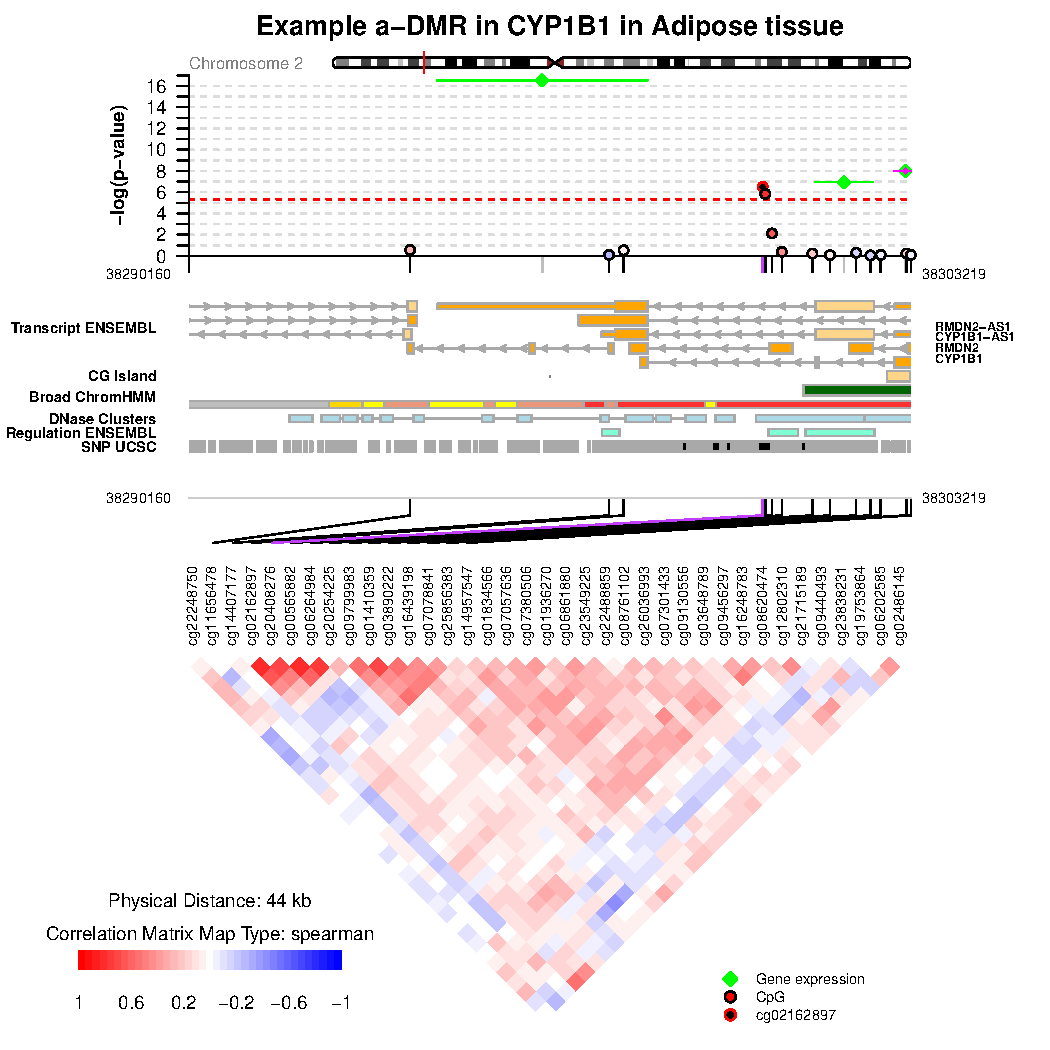
\includegraphics[width=\maxwidth]{figure/minimal-cometwebPlot} 

}



\end{knitrout}
\caption{Plot with comet.web function.\label{fig:cometweb_simple}}
\end{figure}

\section{Creation plot with the generic function: comet}
It is possible to create the annotation tracks by Gviz, trackviewer or ggbio.
Currently, the combinaison of annotation tracks from Gviz with the heatmap of correlation between genetics elements is better plot in coMET.

\subsection{coMET plot: pvalue plot, annotation tracks, and correlation matrice}
\begin{knitrout}
\definecolor{shadecolor}{rgb}{0.969, 0.969, 0.969}\color{fgcolor}\begin{kframe}
\begin{alltt}
\hlkwd{library}\hlstd{(Gviz)}
\hlstd{extdata} \hlkwb{<-} \hlkwd{system.file}\hlstd{(}\hlstr{"extdata"}\hlstd{,} \hlkwc{package}\hlstd{=}\hlstr{"coMET"}\hlstd{,}\hlkwc{mustWork}\hlstd{=}\hlnum{TRUE}\hlstd{)}
\hlstd{configfile} \hlkwb{<-} \hlkwd{file.path}\hlstd{(extdata,} \hlstr{"config_cyp1b1_zoom_4comet.txt"}\hlstd{)}
\hlcom{#configfile <- "../inst/extdata/config_cyp1b1_zoom_4comet.txt" }
\hlstd{chrom} \hlkwb{<-} \hlstr{"chr2"}
\hlstd{start} \hlkwb{<-} \hlnum{38290160}
\hlstd{end} \hlkwb{<-} \hlnum{38303219}
\hlstd{gen} \hlkwb{<-} \hlstr{"hg19"}

\hlstd{genetrack} \hlkwb{<-}\hlkwd{genesENSEMBL}\hlstd{(gen,chrom,start,end,}\hlkwc{showId}\hlstd{=}\hlnum{FALSE}\hlstd{)}
\hlstd{snptrack} \hlkwb{<-} \hlkwd{snpBiomart}\hlstd{(chrom, start, end,} \hlkwc{dataset}\hlstd{=}\hlstr{"hsapiens_snp_som"}\hlstd{,}\hlkwc{showId}\hlstd{=}\hlnum{FALSE}\hlstd{)}
\hlstd{strutrack} \hlkwb{<-} \hlkwd{structureBiomart}\hlstd{(chrom, start, end, strand,}
                              \hlkwc{dataset}\hlstd{=}\hlstr{"hsapiens_structvar_som"}\hlstd{,}\hlkwc{showId}\hlstd{=}\hlnum{FALSE}\hlstd{)}
\hlstd{iscatrack} \hlkwb{<-}\hlkwd{ISCATrack}\hlstd{(gen,chrom,start,end,}\hlkwc{table}\hlstd{=}\hlstr{"iscaPathogenic"}\hlstd{)}

\hlstd{listgviz} \hlkwb{<-} \hlkwd{list}\hlstd{(genetrack,snptrack,iscatrack)}
\hlkwd{comet}\hlstd{(}\hlkwc{config.file}\hlstd{=configfile,}\hlkwc{TRACKS.GVIZ}\hlstd{=listgviz,}
      \hlkwc{VERBOSE}\hlstd{=}\hlnum{FALSE}\hlstd{,} \hlkwc{PRINT.IMAGE}\hlstd{=}\hlnum{FALSE}\hlstd{)}
\end{alltt}
\end{kframe}
\end{knitrout}

\begin{figure}
\begin{knitrout}
\definecolor{shadecolor}{rgb}{0.969, 0.969, 0.969}\color{fgcolor}

{\centering 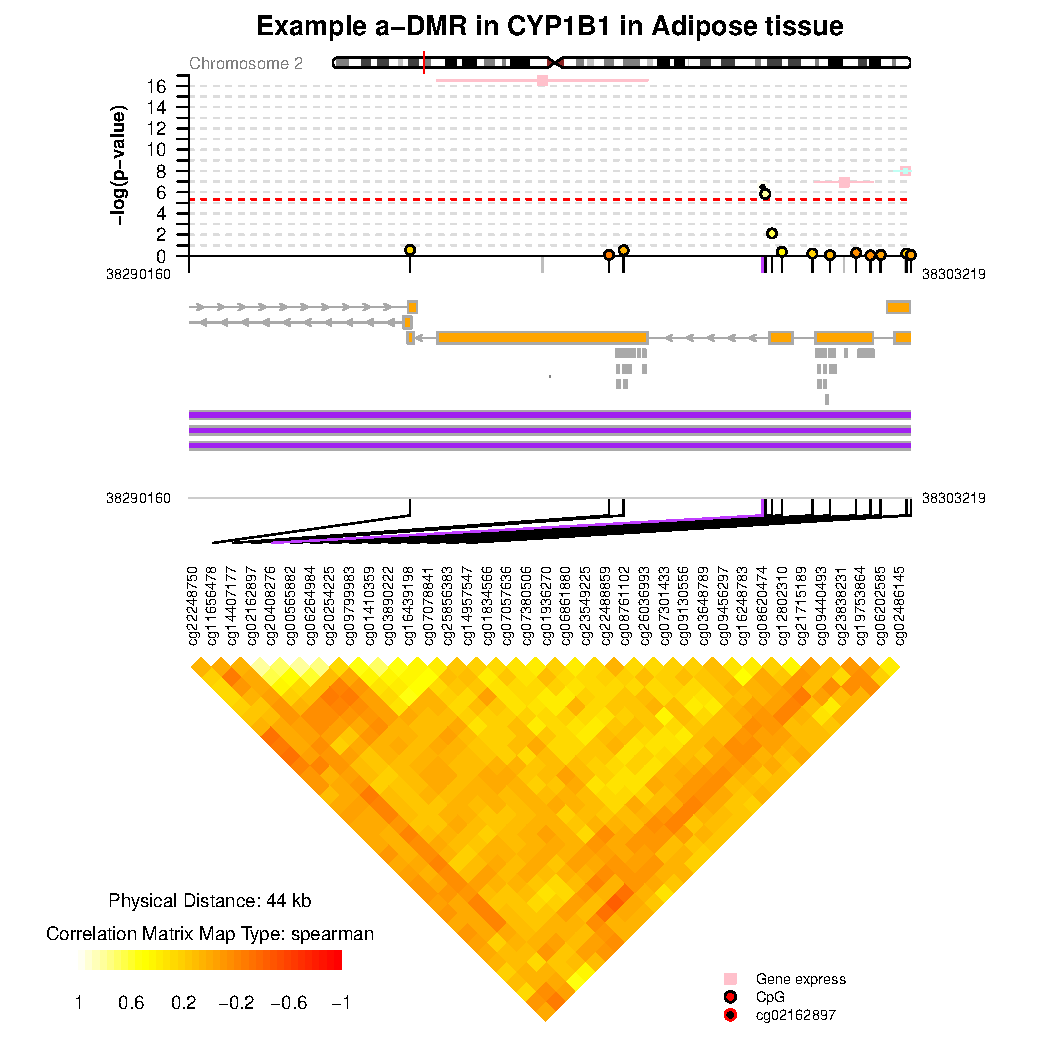
\includegraphics[width=\maxwidth]{figure/minimal-cometPlot} 

}



\end{knitrout}
\caption{Plot with comet function.\label{fig:cometPlot}}
\end{figure}

\subsection{coMET plot: annotation tracks and correlation matrice}  
It is possible to visualise only annotation tracks and the correlation between genetic elements.
In this case, we need to use the option \texttt{DISP.PVALUEPLOT=FALSE}

\begin{knitrout}
\definecolor{shadecolor}{rgb}{0.969, 0.969, 0.969}\color{fgcolor}\begin{kframe}
\begin{alltt}
\hlkwd{library}\hlstd{(Gviz)}
\hlstd{extdata} \hlkwb{<-} \hlkwd{system.file}\hlstd{(}\hlstr{"extdata"}\hlstd{,} \hlkwc{package}\hlstd{=}\hlstr{"coMET"}\hlstd{,}\hlkwc{mustWork}\hlstd{=}\hlnum{TRUE}\hlstd{)}
\hlstd{configfile} \hlkwb{<-} \hlkwd{file.path}\hlstd{(extdata,} \hlstr{"config_cyp1b1_zoom_4comet.txt"}\hlstd{)}
\hlcom{#configfile <- "../inst/extdata/config_cyp1b1_zoom_4comet.txt" }
\hlstd{chrom} \hlkwb{<-} \hlstr{"chr2"}
\hlstd{start} \hlkwb{<-} \hlnum{38290160}
\hlstd{end} \hlkwb{<-} \hlnum{38303219}
\hlstd{gen} \hlkwb{<-} \hlstr{"hg19"}

\hlstd{genetrack} \hlkwb{<-}\hlkwd{genesENSEMBL}\hlstd{(gen,chrom,start,end,}\hlkwc{showId}\hlstd{=}\hlnum{FALSE}\hlstd{)}
\hlstd{snptrack} \hlkwb{<-} \hlkwd{snpBiomart}\hlstd{(chrom, start, end,}
                       \hlkwc{dataset}\hlstd{=}\hlstr{"hsapiens_snp_som"}\hlstd{,}\hlkwc{showId}\hlstd{=}\hlnum{FALSE}\hlstd{)}
\hlstd{strutrack} \hlkwb{<-} \hlkwd{structureBiomart}\hlstd{(chrom, start, end,}
                              \hlstd{strand,} \hlkwc{dataset}\hlstd{=}\hlstr{"hsapiens_structvar_som"}\hlstd{)}
\hlstd{clinVariant}\hlkwb{<-}\hlkwd{ClinVarMainTrack}\hlstd{(gen,chrom,start,end)}
\hlstd{clinCNV}\hlkwb{<-}\hlkwd{ClinVarCnvTrack}\hlstd{(gen,chrom,start,end)}
\hlstd{gwastrack} \hlkwb{<-}\hlkwd{GWASTrack}\hlstd{(gen,chrom,start,end)}
\hlstd{geneRtrack} \hlkwb{<-}\hlkwd{GeneReviewsTrack}\hlstd{(gen,chrom,start,end)}

\hlstd{listgviz} \hlkwb{<-} \hlkwd{list}\hlstd{(genetrack,snptrack,strutrack,clinVariant,}
                 \hlstd{clinCNV,gwastrack,geneRtrack)}
\hlkwd{comet}\hlstd{(}\hlkwc{config.file}\hlstd{=configfile,}\hlkwc{TRACKS.GVIZ}\hlstd{=listgviz,}
      \hlkwc{VERBOSE}\hlstd{=}\hlnum{FALSE}\hlstd{,} \hlkwc{PRINT.IMAGE}\hlstd{=}\hlnum{FALSE}\hlstd{,}\hlkwc{DISP.PVALUEPLOT}\hlstd{=}\hlnum{FALSE}\hlstd{)}
\end{alltt}
\end{kframe}
\end{knitrout}

\begin{figure}
\begin{knitrout}
\definecolor{shadecolor}{rgb}{0.969, 0.969, 0.969}\color{fgcolor}

{\centering 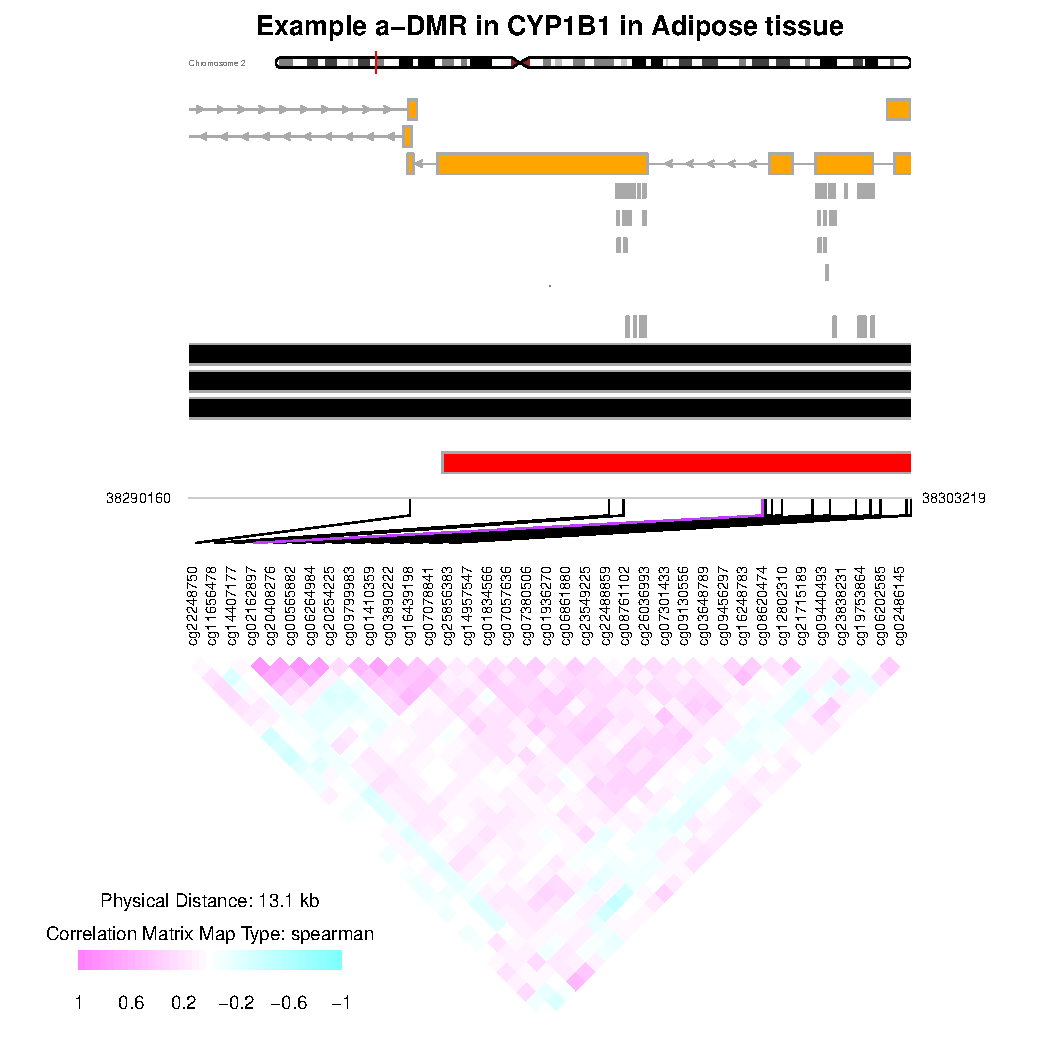
\includegraphics[width=\maxwidth]{figure/minimal-cometPlot_nopval} 

}



\end{knitrout}
\caption{Plot with comet function without pvalue plot.\label{fig:cometPlot_nopval}}
\end{figure}


\clearpage
\section*{SessionInfo}
The following is the session info that generated this vignette:
\begin{kframe}
\begin{alltt}
\hlkwd{toLatex}\hlstd{(}\hlkwd{sessionInfo}\hlstd{())}
\end{alltt}
\end{kframe}\begin{itemize}\raggedright
  \item R version 3.1.1 (2014-07-10), \verb|x86_64-pc-linux-gnu|
  \item Locale: \verb|LC_CTYPE=en_GB.UTF-8|, \verb|LC_NUMERIC=C|, \verb|LC_TIME=en_US.UTF-8|, \verb|LC_COLLATE=en_GB.UTF-8|, \verb|LC_MONETARY=en_US.UTF-8|, \verb|LC_MESSAGES=en_GB.UTF-8|, \verb|LC_PAPER=en_US.UTF-8|, \verb|LC_NAME=C|, \verb|LC_ADDRESS=C|, \verb|LC_TELEPHONE=C|, \verb|LC_MEASUREMENT=en_US.UTF-8|, \verb|LC_IDENTIFICATION=C|
  \item Base packages: base, datasets, graphics, grDevices, grid, methods,
    parallel, stats, utils
  \item Other packages: BiocGenerics~0.10.0, biomaRt~2.20.0, colortools~0.1.5,
    GenomeInfoDb~1.0.2, GenomicRanges~1.16.4, ggbio~1.12.10, ggplot2~1.0.0,
    Gviz~1.8.4, hash~2.2.6, IRanges~1.22.10, knitr~1.6, rtracklayer~1.24.2,
    XVector~0.4.0
  \item Loaded via a namespace (and not attached): acepack~1.3-3.3,
    AnnotationDbi~1.26.0, base64enc~0.1-2, BatchJobs~1.3, BBmisc~1.7,
    Biobase~2.24.0, BiocParallel~0.6.1, BiocStyle~1.2.0, Biostrings~2.32.1,
    biovizBase~1.12.3, bitops~1.0-6, brew~1.0-6, BSgenome~1.32.0, checkmate~1.4,
    cluster~1.15.3, codetools~0.2-9, colorspace~1.2-4, DBI~0.3.0,
    dichromat~2.0-0, digest~0.6.4, evaluate~0.5.5, fail~1.2, foreach~1.4.2,
    foreign~0.8-61, formatR~1.0, Formula~1.1-2, GenomicAlignments~1.0.6,
    GenomicFeatures~1.16.2, gridExtra~0.9.1, gtable~0.1.2, highr~0.3,
    Hmisc~3.14-5, iterators~1.0.7, lattice~0.20-29, latticeExtra~0.6-26,
    MASS~7.3-34, matrixStats~0.10.0, munsell~0.4.2, nnet~7.3-8, plyr~1.8.1,
    proto~0.3-10, RColorBrewer~1.0-5, Rcpp~0.11.2, RCurl~1.95-4.3, reshape2~1.4,
    R.methodsS3~1.6.1, rpart~4.1-8, Rsamtools~1.16.1, RSQLite~0.11.4,
    scales~0.2.4, sendmailR~1.2-1, splines~3.1.1, stats4~3.1.1, stringr~0.6.2,
    survival~2.37-7, tools~3.1.1, VariantAnnotation~1.10.5, XML~3.98-1.1,
    zlibbioc~1.10.0
\end{itemize}

\end{document}
